\documentclass[UTF8,a4paper,11pt,fontset=none]{ctexart}
\usepackage{fontspec}\setmainfont{Times New Roman}\setsansfont{Arial}\setmonofont{Menlo}\setCJKmainfont{Songti SC}\setCJKsansfont{Heiti SC}
\usepackage[margin=2.2cm]{geometry}\usepackage{amsmath,amssymb,graphicx,booktabs,tabularx,hyperref,microtype}
\hypersetup{hidelinks}\setlength{\parskip}{.4em}\setlength{\emergencystretch}{2em}
\title{接收电流空间何时值得改变？\\关于材料激发、内部反馈与条件交换的研究汇报}
\author{}\date{}
% Use cached readable math sizes; no network font installation.
\DeclareMathSizes{10}{10}{7}{6}
\DeclareMathSizes{9}{9}{6}{6}
\DeclareMathSizes{8}{8}{6}{6}
\DeclareMathSizes{7}{7}{6}{6}
\DeclareMathSizes{6}{6}{6}{6}
\DeclareMathSizes{5}{6}{6}{6}
\begin{document}\maketitle\vspace{-1.5em}
陈教授您好，我想汇报一个从电流压缩引出的材料反演问题。我最初希望用高斯（Gaussian）材料表示和少量电流端口降低计算量，后来发现，比“压缩后的场是否足够准确”更关键的是：这些电流方向生成的材料更新是否正确。现在我把问题收窄为：已有一个通过端点求解检查的接收电流基底，什么时候值得换掉其中一个方向？

\section{文献背景与问题的来由}
电磁逆散射（electromagnetic inverse scattering）根据外部散射场估计内部介电材料。感应电流（induced current）连接材料与测量：材料在总场作用下产生电流，电流通过内部Green算子相互作用，最后向接收器辐射。求解器若保留全部电流自由度，三维计算和反演线性化都很昂贵，所以电流子空间（current subspace）自然成为组织问题的方式。

我对subspace-based optimization method（SOM，子空间优化方法）的理解是，它首先利用接收Green算子的奇异结构区分容易观测和较难观测的电流，再结合材料与电流的一致性求解。Twofold SOM（TSOM）进一步利用内部传播；FFT-TSOM利用Fourier结构组织更高效的电流空间。Subspace-based distorted-Born iterative method（S-DBIM）则把背景更新与电流信息结合。因此，我想补上一个具体接口：\emph{在给定材料和当前残差下，改变这个电流子空间，会怎样改变材料这一步？}

输出保持、导数保持和目标导向降阶模型（output-/derivative-preserving and goal-oriented reduced-order model, ROM）已有丰富研究；Krylov方法也直接围绕材料方程构造有效方向。我关注的物理链条是材料激发怎样进入指定电流、内部反馈怎样改变它的接收返回，以及这个改变怎样作用于当前材料步。这些已知方法是比较的出发点，指定电流替换的材料后果才是我想算清楚的接口。

\section{材料扰动先变成电流激励，再经过多重散射}
对第$p$次照明，用$\chi$表示材料对比度，$Q_Ts$表示允许的微小材料变化。$s$是实材料坐标，复介电常数的实部和虚部都在其中；$Q_T$在体积加权材料度量下正交化。材料方向经过当前总场形成注入（material injection）$B_ps$，再经完整内部方程$L$得到电流变化：
\[
L\,\delta j_p=B_ps,\qquad J_p=SL^{-1}B_p.
\]
$S$是接收及测量归一化算子。材料、局部总场、照明和材料表示都进入$B_p$。实际离散偶极子近似（discrete-dipole approximation, DDA）使用极化率（polarizability）$a(\chi)$，注入包含$a'(\chi)e_p^{\rm tot}$；极化率与材料对比度通过这个离散关系相连。各照明有自己的电流，但共享同一个材料变量，伴随必须做正确的实材料拉回（real material pullback）。

\section{新增电流有直接辐射和保留反馈两条路径}
设$V$是保留基底，$C$是指定新增方向，$R_0=V(V^*LV)^{-1}V^*$。取电流形式$L=I-XG_D$：$X$是同一电流归一化下的材料乘法算子，$G_D$把电流映射成内部场。在DDA离散中需使用相应极化率及自作用约定。消去$V$中的坐标以后，新增方向变成
\[
\bar C=(I-R_0L)C=C+R_0XG_DC.
\]
第一项是新增电流本身；第二项是它产生内部场、激发保留电流，后者再经过保留空间散射返回的响应。这是频域反馈（frequency-domain feedback），来自方程消元。接收器看见$S\bar C$，而不只是$SC$。

\begin{figure}[htbp]\centering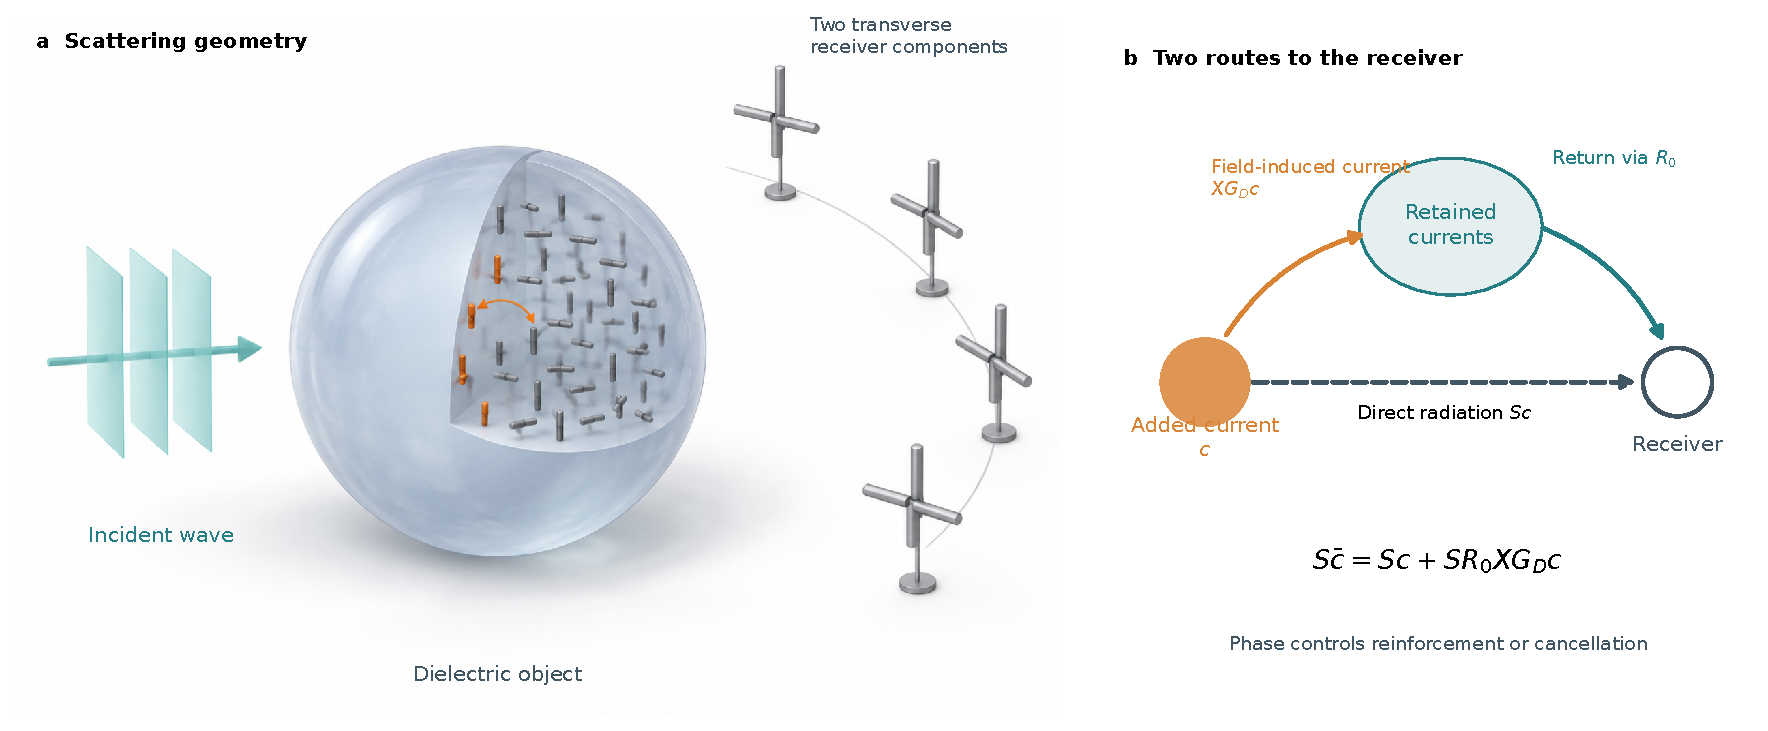
\includegraphics[width=.94\linewidth]{figures/physical_feedback.pdf}
\caption{新增电流的直接辐射和保留电流反馈。场景是概念示意；箭头不代表计算场分布。}
\end{figure}

令$Y_C=S\bar C$为反馈后的观测因子，$N_C=C^*(B-LR_0B)$为材料进入新增方程的有效激励，$\Gamma_C=C^*L\bar C$为Schur补。端点导数差精确写成
\[
D_C=J_C-J_0=Y_C\Gamma_C^{-1}N_C.
\]
$Y_C$说明作用能否返回接收器，$N_C$说明当前材料扰动能否激发它；$\Gamma_C$保留两空间之间的反馈耦合。直接接收强度无法单独代替这个乘积。一个受控三维例子中，直接输出低于$1.7\times10^{-16}$，反馈后输出却为0.0672--0.0888，指定增广的材料导数变化达到3.56--5.22\%。

\section{通路完整不等于当前材料步有收益}
冻结当前材料、残差$r$、共同正则曲率$\Lambda$和先验线性项$\ell$后，正则化Gauss--Newton（GN）材料法方程为
\[
H_Us_U=-h_U,\qquad H_U=J_U^TJ_U+\Lambda,\quad h_U=J_U^Tr+\ell.
\]
记原端点的材料法方程矩阵为$H_0=J_0^*J_0+\Lambda$。对指定增广，我可以证明步差落在两组材料方向组成的空间：
\[
s_C-s_0\in\operatorname{Range}H_0^{-1}[J_0^*Y_C,N_C^*].
\]
这里$Y_C,N_C$在材料空间公式中也按全部照明实化：不同照明有不同电流分量，但共享实材料变量。第一组通过原敏感度把新增接收响应带回材料，第二组通过新增激励把残差带回材料。这个双侧支撑（paired material support）解释步会在哪里改变；它并没有判断这种改变是否对当前完整目标有用。

改变电流模型，同时改变数据曲率$\mathsf I=J^TJ$和残差拉回$h=J^Tr+\ell$。对新旧端点，实际步差为
\[
d=s_n-s_o=-H_n^{-1}(\Delta h+\Delta\mathsf I s_o).
\]
这里两项要共同看。电流空间变大是在改变已有数据的近似模型，曲率增量可以不定。为了检验“响应更强是否就更有用”，我使用两个常见汇总量：信息体积（information volume）把尺度归一化曲率的特征值$\nu_i$汇总成$\tfrac12\sum_i\log(1+\nu_i)$；有效维数（effective dimension）用$\sum_i\nu_i/(1+\nu_i)$描述显著响应方向的数量。这里$\nu_i$来自$P_0^{-1/2}J_U^TJ_UP_0^{-1/2}$，固定$P_0=10^{-5}I$，与求解时为控制步长而加入的Levenberg--Marquardt（LM）阻尼分开。这两个数压缩了曲率信息，却没有保留当前残差的方向。

真实Maxwell替换中，我看到信息体积增加6.3127、有效维数增加1.8613，相对完整曲率的归一化误差还略有下降，完整GN收益却为负。另一个增广见证中，两列单独加入都不利，联合加入却有利，说明作用需要放在当前空间中判断。对共同候选的受控比较，我暂时关闭no-op并强制选一个候选：只看实际位移的线性收益，29/36次选到负收益；计入有限位移的二次代价后降到1/36。这是解释排序的诊断，实际部署仍保留接受复核和no-op。

历史对照也帮助我区分了两件事。沿完整描述步差的两组材料方向作双侧材料修正（paired repair），在72个平滑及36个尖锐冻结比较中都优于对应的直接电流增广（direct current enlargement）。但等材料秩的Krylov修正全部更好，计入构建与检查后的paired路径耗时为匹配预条件共轭梯度（preconditioned conjugate gradient, PCG）的1.416倍。由此我选择用电流结构判断模型如何改，而不是让它替代完整材料求解器。

\section{我采用的设计：接收基底上的条件交换}
我从接收导出的起始基底（receiver-derived basis）出发，检查一列移出、一列移入的具体替换。保留的是电流总维数，原receiver列可以被换掉。较丰富的约化参考（richer reduced anchor，简称anchor）先排序，每轮最多对两个进入完整复核的候选（finalist）做$Jd$检查，最多接受三个动作；没有可靠正收益时就保持当前空间。接受以后重新计算条件耦合，不能把第一次得分沿用到底。相同电流维数让我们比较表示的材料用途，额外anchor、候选取得与完整检查的费用也同时保留。

判断标准是实际位移在共同完整二次目标上减少了多少。令$x=s_o$为当前约化模型生成的材料步，$F$指共同完整二次模型，$g_F(x)$和$H_F$是它的梯度与曲率：
\[
Q=-g_F(x)^Td-\tfrac12d^TH_Fd.
\]
缓存$u=r+J_Fx$，只算$z=J_Fd$即可评价
\[
Q=-\operatorname{Re}\langle u,z\rangle-(\ell+\Lambda x)^Td
-\tfrac12(\|z\|^2+d^T\Lambda d).
\]
这样每个finalist只增加一个材料方向在全部照明下的切向作用，不需要再计算完整伴随，也不需要完整最优材料步$s_*$。这个作用仍需收费。

接受阈值仅依赖上述各项的在线尺度、FP64精度和预先固定的常数；原完整参考底噪已从controller移出。36单元真实回放中，75个接受动作、终态空间、材料步和风险保持完全一致。这是高精度数值复核（high-fidelity numerical verification），尚未实例化严格输出误差半径，所以我不用deterministic certificate描述它。

\section{冻结规则以后，材料步改善是否仍然出现}
我先用平滑Gaussian、近接触Gaussian、分层体素（voxel）和非对称voxel四个对象检查方法，分别取初始化、保存迭代索引3和最后保存的状态，再比较$k=4,8,16$。这36个单元中35个改善、1个保持相同；四个对象先各自求和再比较，中位完整GN gap下降65.2\%。这里九个状态和预算组合仍属于一个对象，我没有把它们当成九个独立样本。

随后我锁定全部规则和数值阈值，检查资产中其余所有兼容对象。十个对象完整提供各九个单元，十个都改善；中位风险比0.4928，即下降50.7\%，四分位区间[0.3314,0.5588]。按对象重采样（object bootstrap）得到的中位数95\%区间为[0.3133,0.5647]。还有一个非对称voxel对象的中期以前六个单元改善，但晚期receiver endpoint在第一个预算没有通过预设法方程残差（normal residual）检查，后面两个预算未运行。因此预定99个单元只有96个有有效结果，失败仍在总表中。

\begin{figure}[htbp]\centering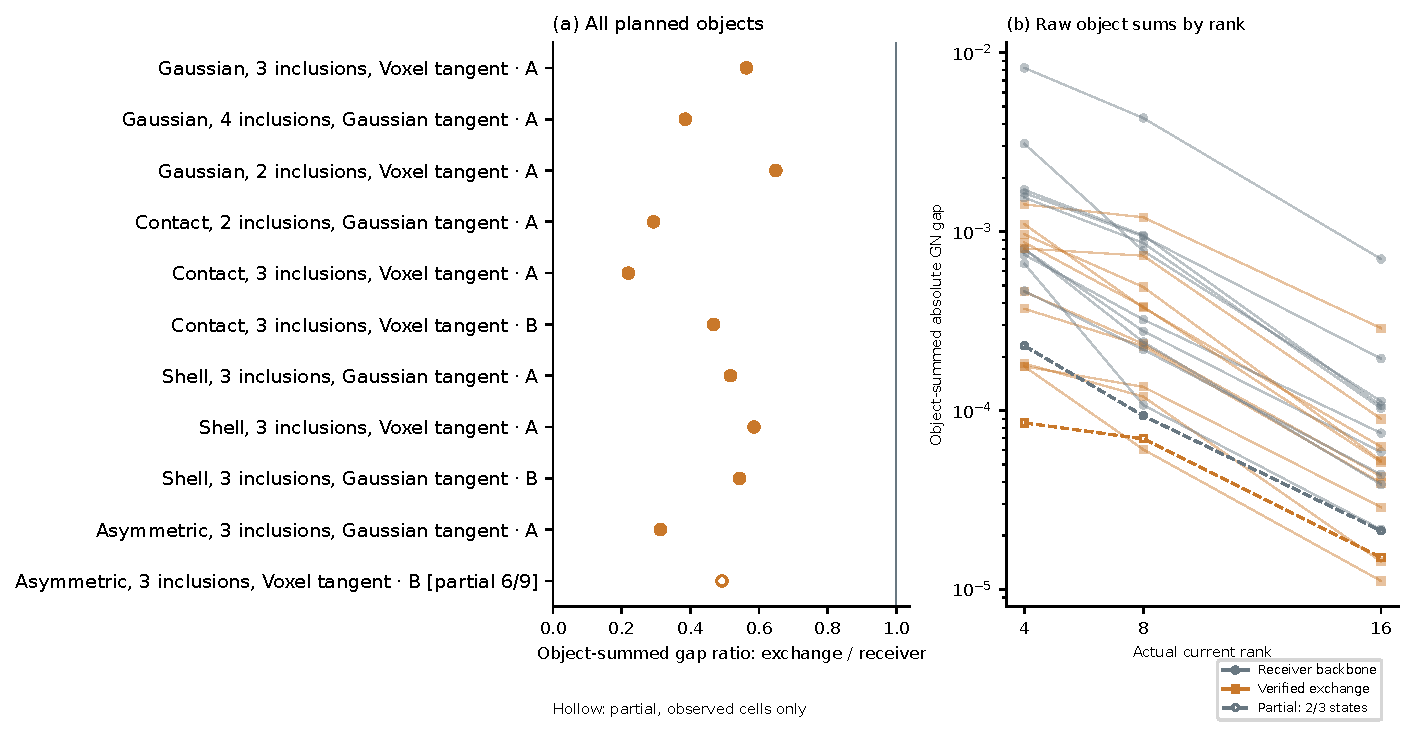
\includegraphics[width=.96\linewidth]{figures/closure_validation_v2/Figure1_primary_overview.pdf}
\caption{左图逐对象展示完整GN gap之和的比值，右图展示不同实际电流秩下的绝对gap。空心点和虚线单独标出只有六个可用单元的对象。这张图检验材料步保真度，不是最终材料图像。}
\end{figure}

这个结果比较有说服力的地方是，效果不只来自原四个对象，也不只来自小分母：最小receiver gap仍超过evaluation floor约$6.31\times10^9$倍。96个有效单元中95个改善、1个相同，绝对下降量和$H$范数步误差都有逐项记录。不过，这些对象曾进入宽域current-ranking研究，无法确认它们完全没有影响过历史规则判断。因此我把它们称为冻结规则在额外对象上的检验，避免把它写成全新blind dataset。

\section{加噪声以后，收益保留，但电流方向会改变}
我按几何和材料表示事先选了四个对象：平滑voxel、接触Gaussian、壳体Gaussian和非对称voxel。固定中期物理状态，在1\%和3\%复噪声下各用三份独立噪声样本（realization），再比较三个电流秩。每份噪声都有自己的完整GN reference，因为残差改变，材料步的比较目标也随之改变。

72个单元全部完成，71个改善、1个保持原空间。四对象汇总风险比的中位数在1\%时为0.3307，在3\%时为0.4026。这个有限噪声测试支持材料步收益仍然存在。它没有要求选择同一组电流：用主角度（principal angle，衡量两个物理子空间的偏离）比较保存的空间，很多补入方向明显改变。因此更合适的理解是，方法追随当前残差选择有用的变化，而不是得到一个不随数据改变的稳定模式表。

完整复核检查408个finalist，其中98个低于数值接受阈值，共接受172次交换。Jd核验用了2448个电流方程右端（current right-hand sides, RHS），包括被拒绝的候选。已有缓存后的评分（warm scoring）只是其中一个阶段，完整费用还包括取得候选与物理检查。

\subsection{好方向是否进入了候选池？}
为了区分“评分不准”和“没有送来好候选”，我在已完成线上决定以后，离线枚举固定154方向字典中的全部初次一换一机会（initial one-exchange opportunity），再走最多三个按完整收益选择的局部动作。这个teacher只作诊断，没有回传到线上规则。96个可用单元完整，之前端点失败对应的3个单元仍未运行。

在十个完整额外对象中，如果允许anchor在全字典排序，它保留的初次正收益机会为97.30--99.99\%，中位99.54\%。但是固定12个移入候选的短池只覆盖49.12--95.31\%，中位72.95\%。这些比例先对对象内机会求和，因此我把目前更明显的瓶颈理解为候选取得（candidate acquisition），而不是排序公式本身。这并不表示已经解决全局选模：后续交换进入不同条件空间，局部路径也会不同。完整收益贪心路径在90个单元终态更好，线上路径在5个单元更好，1个在评价底噪内相同；这个差距包含覆盖、排序与路径共同作用。


\subsection{把规则放回真正的约束反演以后}
我还固定四个代表对象，把receiver和exchange放进相同的outer reconstruction：同一初始化、prior、LM schedule、材料可行域以及完整非线性目标上的Armijo line search，只改变切向电流策略。三个完整对照都完成18次接受更新。平滑voxel、近接触Gaussian和shell Gaussian的复材料相对误差分别从0.3027、0.6722、0.6096降到0.2699、0.6707、0.5660，约下降10.8\%、0.22\%、7.16\%。留出测量误差也均下降。

这里有一个值得正面解释的差别：近接触对象的数据拟合改善很明显，但复材料改善很小，实部还略差。这使我更明确地区分“更忠实的完整GN步”和“更好的材料估计”。第四个非对称voxel对象的exchange轨迹保留17次已完成更新。在第18次更新前，它为开始当次交换构建的receiver endpoint没有通过残差验收，因而停止；独立的receiver-only基线轨迹尚未运行。我保留这组未形成完整对照的结果，没有放宽验收条件。

每条轨迹独立计入setup、acquisition、line search和最终评价后，exchange耗时是receiver的2.68、1.74、1.46倍。它支付了额外的$Jd$作用，换取更新保真度，而不是更快的成像。我的论文因此以Maxwell机制和conditional design为主，把这三组重建作为有限的secondary consequence。

\begin{figure}[htbp]\centering
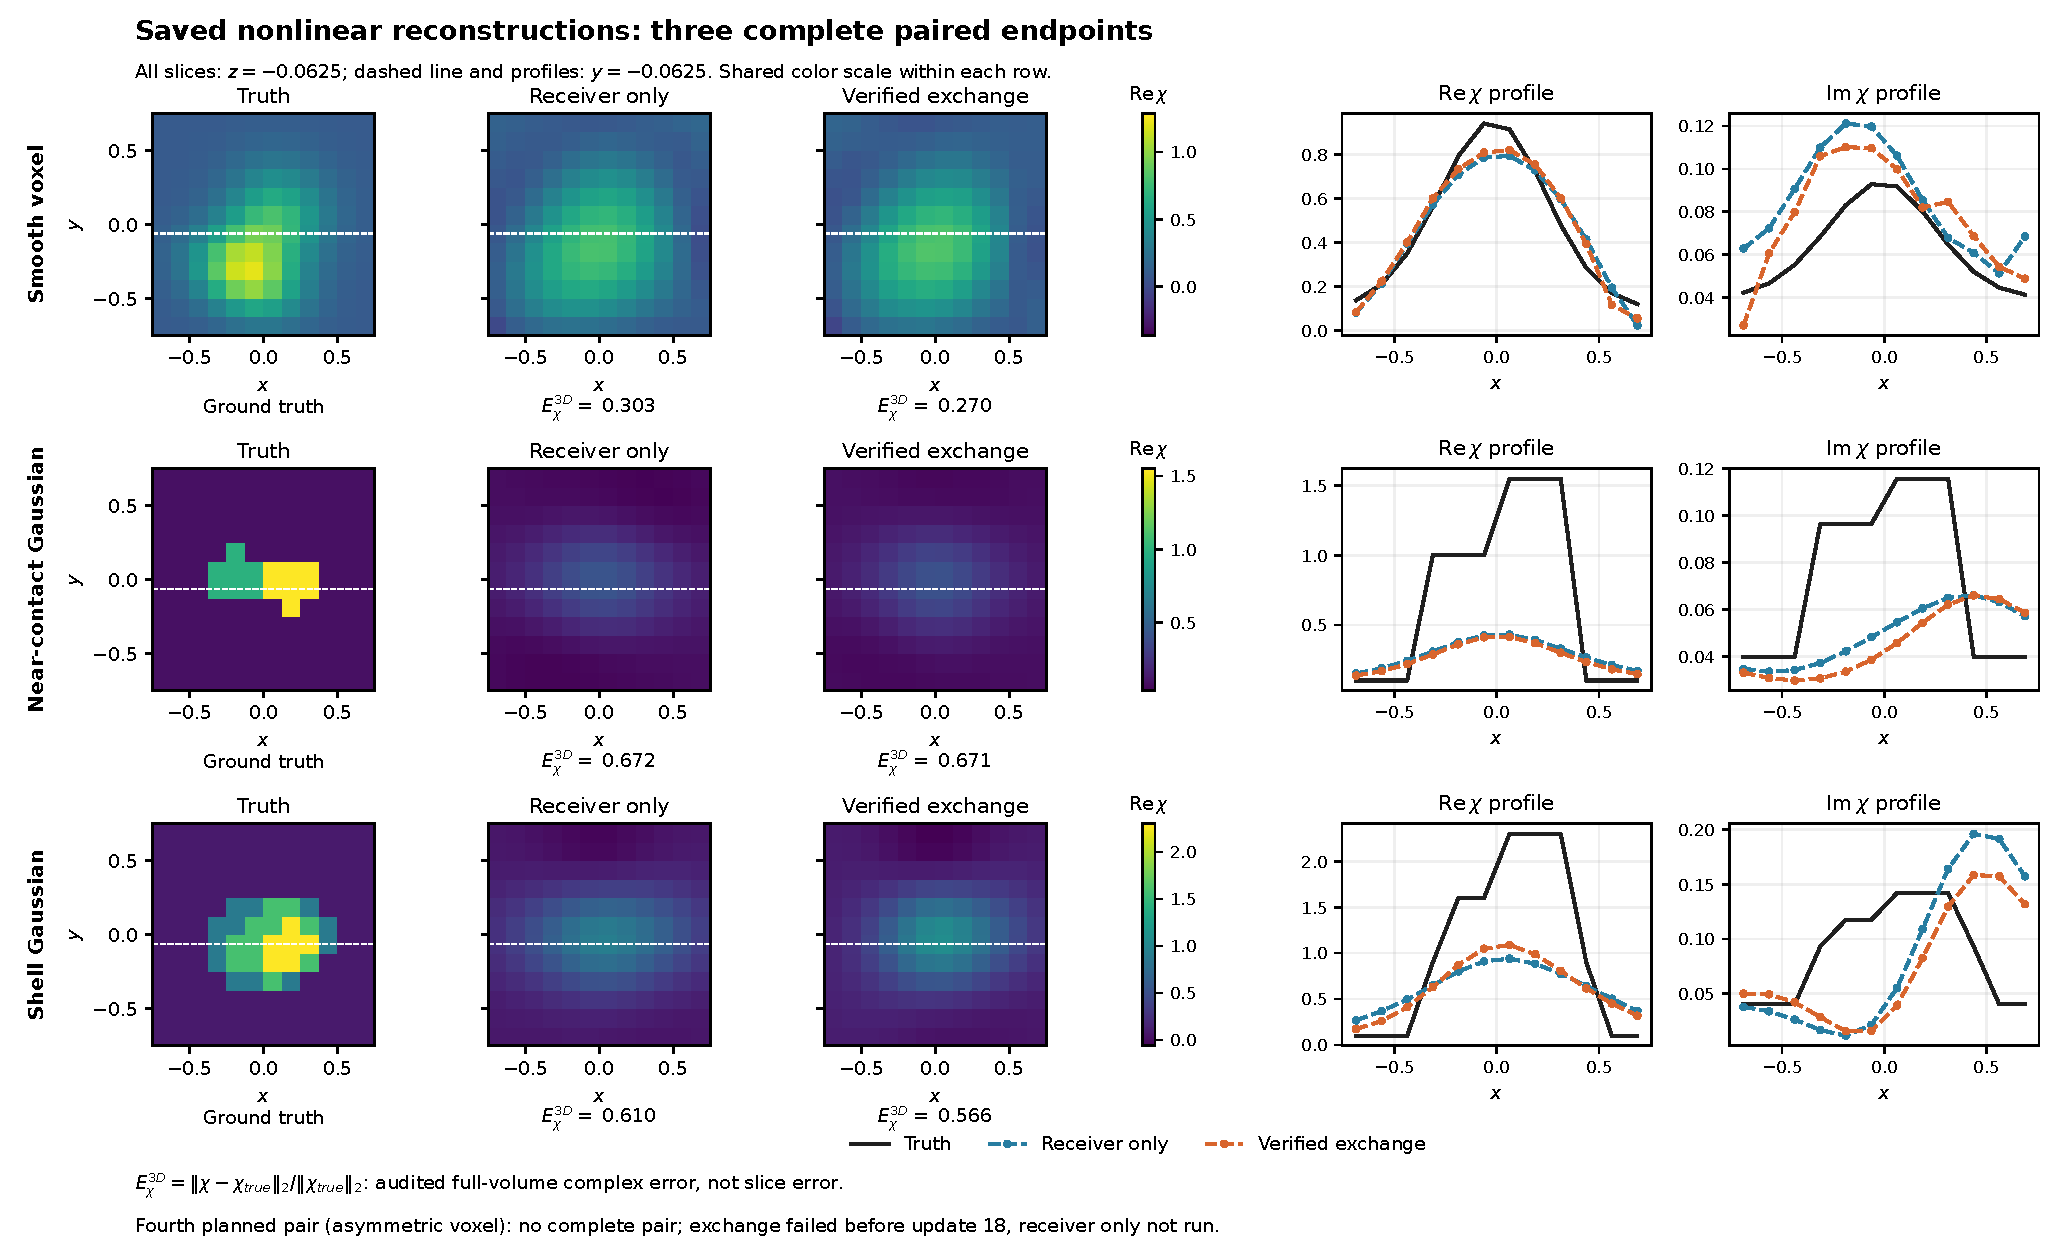
\includegraphics[width=.95\linewidth]{figures/nonlinear_closure_v1/nonlinear_reconstructions.pdf}
\caption{三组完整对照的材料切片与剖面。每行共用色标，曲线同时展示实部和虚部；完整误差用整个三维材料计算。近接触及shell结构的峰值和界面仍不清晰，数据拟合改善没有自动解决材料辨识。}
\end{figure}


\subsection{改善的代价如何理解}
我把费用分成共同物理计算、anchor与候选取得、排序、完整方向核验、离线诊断和真正重建，拒绝动作和失败也计入。整个研究的已计费作业占用为5.545小时；这个数是执行账本，不能当成一次反演的时间。冻结流程重用共同算子，数秒的warm选择也不能代表冷启动。

三对独立重建的exchange耗时为receiver的2.68、1.74和1.46倍。因此我的结果是用额外物理作用换取材料步保真度，并在部分对象看到有限重建后果。它没有给出加速成像结论。每个finalist的复核只需要完整$Jd$，省掉的是这项判断中的新增伴随（adjoint），并没有省掉取得候选和验证所需的全波计算。




\section{我对结果的理解，以及想请教的问题}
我的理解是，接收可见性提供一个可靠的起点，材料激发和内部反馈解释某个替换能产生什么影响，残差相关的有限收益才判断这个影响现在是否值得。这个链条把物理通路与材料更新连起来，而不是寻找一个脱离状态和目标的普遍模式排名。

我想请教两个物理和方法上的问题。第一，在SOM/TSOM已有的内部传播组织中，您会如何理解这个保留空间返回项？特别是直接辐射接近零时，哪些几何或材料条件最有可能让反馈路径成为主导，哪些条件会使它抵消？第二，面对短候选池漏掉有用方向的情况，您觉得怎样的物理构造最适合扩大有效候选覆盖，而不先支付很大的全波费用？我希望把这个问题作为后续工作的具体起点，而不是不断叠加一个更复杂的求解器。

\section*{主要阅读线索}
陈教授的\emph{Computational Methods for Electromagnetic Inverse Scattering}及已取得全文的子空间方法综述，是我理解既有传播机制的主要依据。Primal/dual inverse ROM原文提供导数保持的对照。SOM、TSOM、FFT-TSOM及S-DBIM原始论文的全文仍有缺口；完整书目、全文证据和这些未关闭的条目随补充材料说明。因此论文采用明确的机制比较，不作历史优先性宣称。
\end{document}
